\documentclass[11pt,letter,oneside]{report}
\usepackage[pdftex]{graphicx}
\begin{document}

\title{Space Invaders}
\author{Peter Hamilton and Jared Pilcher}
\date{Fall 2011}
\maketitle

\tableofcontents

\chapter{Space Invaders Overview}
\section{History of Space Invaders}

Designed by Tomohiro Nishikado in 1978, Space Invaders is one of the greatest arcade games of all time. It took Nishikado over a year to develope the game and its hardware. It was manufactured in Japan by Taito. It was so influential that it pushed the video game industry into a worldwide industry. Shortly after its release, it caused a shortage of 100-yen in Japan. By 2007, Taito earned over \$500 million dollars in profits. 

Space invaders was a really popular game in 1978. It is one of the most influential and successful games of all time. It is a two dimensional shooting game involving a tank that shoots aliens marching across a screen. When all of the aliens were destroyed, or all of the lives of the tank were used, the game ended. It has had several sequels, and was released on several platforms. It was the inspiration for many other video games on the market today. 

To this day, a bug still exists from the original game. In the original game, as the marching aliens were killed, the game refreshed faster since there was less to load an the screen. This added an extra challenge to the game. As the game became popular, consumers became accustomed to the bug. When the developer fixed the bug, the market responded poorly. It was placed back into the game, and has been there since.
 
\section{Game Play}

\subsection{Objective}

The world is being invaded by marching aliens.  All of humanity has gathered behind 4 bunkers for protection.  You control the only weapons available, a supply of 3 tanks and a handful of missiles. Kill all the aliens! Watch out! The alien mothership flies over head! Destroy it at all costs!  The fate of the world rests in your hands...

Win the game by killing all of the marching aliens. Destroying the mothership gives you extra points.

\subsection{The Tank}
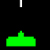
\includegraphics[]{tank.jpg}

You are the tank. Push the left button to move left, and the right button to move right. You can fire and move simultaneously.

Watch out! Enemy fire rains from above! Dodge the alien fire by moving the tank left or right. Each time your tank is hit by an alien bullet, it explodes. You have three lives.  You must survive...

Fire your missile to destroy the alien invaders! Push the middle button to fire your missile, aiming for the aliens. When the missile hits an alien, it dies. Be careful! They move left and right, and get closer as time goes on.

\subsection{Enemies}

\subsubsection{Spaceship}

\includegraphics[]{big-alien.png}

The alien mothership circles the Earth, looking for its prey. Destroy it at all costs! It flies occasionally from left to right. As it flies overhead, launch your tank missile by pushing the middle button. Be careful, it tries to evade you missile, so shoot accurately and quick!


\subsubsection{Aliens}

\includegraphics[]{aliens.jpg}

55 aliens are marching toward your position! You are charged with destroying all of them before they reach you! Fire your missiles to kill them! These aliens can shoot up to four bullets at a time. 

Aliens are capable of destroying walls, so your bunkers will provide no protection when they reach them. Their bullets slowly degrade your bunkers when they're hit. Be quick! You will soon have no protection!

\subsection{Points}
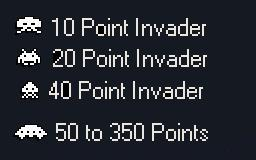
\includegraphics[]{scoring.jpg}

Earn points by destroying the aliens with your tank missiles. The lower two rows of aliens, middle two rows of aliens, and the top row of aliens are worth 10, 20 points and 40 points per alien, respectively.

Earn extra points for destroying the mothership! Earn between 50 to 350 points for each mothership destroyed.

\section{Game Details and Specifications}

\subsection{Aliens}

\subsubsection{Alien Placement and Appearance}
There are 55 aliens that start on the screen.  They are on a 11 by 5 grid.  Each grid is 15 pixels by 15 pixels.  There are three types of aliens.  The first two rows are the widest aliens, the next two rows are a little narrower and the top row has the narrowest alien.

\subsubsection{Alien Movement}
The aliens move laterally in increments of 2 pixels.  When the rightmost aliens reach the right edge of the screen, the grid of aliens will move down 7 pixels and start moving left.  When the leftmost aliens reach the left edge of the screen, they will move down 7 pixels and start moving right.  The rightmost alien and leftmost alien is the closest alien to the respective sides that has not been killed. This means that when the rightmost column of aliens are destroyed, the aliens march toward the side of the screen until the next column hits that side. The aliens continue this pattern of movement until the bottommost row of alive aliens reaches the bottom of the bunkers. The aliens will speed up in their movement as aliens are killed.

\subsubsection{Alien Explosions}
When an alien is hit by a bullet from the tank, it blows up.  The other aliens continue onward while the explosion sequence is happening.

\subsection{Alien Mothership}
The alien mothership flies across the screen from left to right. It's time of appearance is random. When a bullet strikes the mothership, it flashes, revealing the score received.

\subsection{The Tank}
\subsubsection{Movement}
The tank moves laterally across the bottom of the screen. The user is able to push the right button to move right, or push the left button to move left at a rate of two pixels. The user is able to hold down the left or right buttons to keep the tank moving across the screen.
\subsubsection{Firing Bullets}
You may also fire a missile by pushing the middle button. The tank is capable of moving and firing simultaneously. It is also capable of changing direction while shooting. This means that you are able to hold down the fire button and change directions.
\subsubsection{Death}
When the tank is struck by an alien bullet, it explodes.  The player will lose a life and continue the current level.

\subsection{Bullets}
\subsubsection{Tank Bullets}
Tanks are capable of firing bullets by pushing the middle button. Tank bullets, unlike Alien Bullets, only have one appearance. They are white rectangles that are ejected just above the center of the tank. No black boxes surround the bullet. In other words, when it leaves the tank, or strikes an object, an overlay of a black box cannot be seen. 

When a bullet is on the screen, the tank cannot fire again until the bullet has left the screen. Each bullet travels at a rate of 2 pixels. When it strikes an alien or mothership, the object is destroyed.

\subsubsection{Alien Bullets}
There are two types of alien bullets:
\begin{enumerate}
\item{}  Zig zag bullets rotate cyclically through the following appearances:

\begin{enumerate}
\item 
 
\includegraphics[scale=2]{ZigBullet0.png}
\item 
 
\includegraphics[scale=2]{ZigBullet1.png}
\item
 
\includegraphics[scale=2]{ZigBullet2.png}
\item
 
\includegraphics[scale=2]{ZigBullet3.png}
\end{enumerate}

\item{}  Cross bullets oscillate through the following appearance:

\begin{enumerate}
\item
 
\includegraphics[scale=2]{TBullet0.png}
\item
 
\includegraphics[scale=2]{TBullet1.png}
\item
 
\includegraphics[scale=2]{TBullet2.png}
\end{enumerate}

\end{enumerate}

Each bullet is ejected from the center of an alien, randomly chosen to be an alien on the bottommost row. There can only be 4 bullets on the screen at any given point in time.  Once a bullet leaves the screen, a new bullet can be fired. Each bullet travels at a rate of 2 pixels. When the bullet strikes a tank, it is destroyed. When the bullet strikes a bunker, the bunker is eroded. When a piece of the bunker is completely eroded, the bullet can pass through it.  No black boxes surround the bullet. In other words, when it leaves an alien, or strikes an object, an overlay of a black box cannot be seen. 

\subsection{The Bunkers}
There are four bunkers available for the tank to use as cover.  Each bunker is divided into 10 sections.  Each section partially erodes with each collision of an alien bullet.  After 4 collisions, the section is fully eroded and will allow bullets to pass through.

When the aliens reach the bunkers, they will walk above the bunkers as they move through them. In other words, they will be drawn over the bunkers and those portions of the bunkers will be destroyed.


\subsection{Scoring}
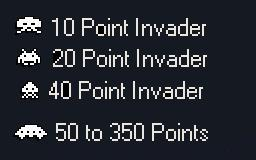
\includegraphics[]{scoring.jpg}

Earn points by destroying the aliens with your tank missiles. The lower two rows of aliens, middle two rows of aliens, and the top row of aliens are worth 10, 20 points and 40 points per alien, respectively.

\subsection{End of Game}
The game ends when one of the following three events occur:
\begin{enumerate}
\item The bottommost row of aliens that are alive reach the bottom of the bunkers.
\item The tank has been destroyed three times.
\item All aliens are destroyed.
\end{enumerate}
When the game ends, a game over screen is displayed.

\subsection{Appearance}
The game appearance is identical to the flash version of Space Invasion. The game runs smoothly and at a decent speed. The screen is also updated close to the same rate as the flash-based game. No artifacts appear on the screen. No flickering occurs on the screen.

\chapter{Bug Reports and File Organization}

\section{Bug Reports}

\subsection{Drawing Bullets}
During our design phase, we found a bug involving the drawing of alien bullets to the screen. 

First, we had difficulty cycling through the different different stages of the bullet. We were able to cycle through four stages, however, the fourth state was a different bullet type entirely. We fixed the bug by placing a simple if statement in our draw bullet loop. When the bullet was in the fourth stage, it cycled back to the third state to and reset its state to the first state. In this way we were able to use the same functions for a four cycle bullet and a three cycle bullet.

Second, we found a bug when the first bullet was fired. Without permission, another bullet was drawn at pixel location (0,0). We found the problem by analyzing our bullet structs. We discovered that our bullet variables were not initialized to zero. We assumed that they would be initialized to zero, but a random value was placed there. When we initialized all variables, the bug was fixed.

\subsection{Destroying Aliens}
During our design phase, we found a bug involving the destroying of aliens. We thought that the lab instructions said to give find a random number between 0 and 54 and destroy that alien. When we tried to pass it off, the TA told us that we needed to ask the user to input a number. To fix the bug, we used the read() function to acquire a number from the user, one integer at a time. We destroyed the alien that corresponded to that number.

\subsection{Moving Aliens to Right of Screen}
We initially had some naive logic concerning the aliens reaching the edge of the screen.  We set a hard limit for the grid of aliens.  Once the top left corner of the grid had reached the limit, the aliens moved down and changed directions.  This did not account for all aliens on the edge of the grid being dead, which would require the alien grid to move one column closer to the edge than it did with all aliens alive.  We fixed this by using a more dynamic approach.

\subsection{Overlay of Bullet Black Boxes}
During our design phase, we found a bug involving the overlay of the bullet black boxes. We discovered that as a bullet was launched, and flew over objects on the screen, it had black boxes surrounding it. We have not yet resolved this bug, but will do so in the near future.

\subsection{One Alien Firing Two Bullets Simultaneously}
While trying test our implementation of aliens firing bullets, we encountered a situation in which an alien fires two bullets on top of each other.  They will appear as one bullet.  We solved this by limiting the firing of a bullet until the first one has moved out of its original position. 
\end{document}